\documentclass[journal]{IEEEtran}
%\usepackage[utf8]{inputenc}

\usepackage{graphicx}
\ifCLASSINFOpdf
\else
\fi
\usepackage{url}
\usepackage{amsfonts}
\usepackage[noadjust]{cite}
\renewcommand{\citepunct}{,\penalty\citepunctpenalty\,}
\renewcommand{\citedash}{--}% optionally

\hyphenation{op-tical net-works semi-conduc-tor ns- however}

\title{Blockchain-enabled Network Sharing for O-RAN}

\author{Lorenza Giupponi and Francesc Wilhelmi\thanks{The authors are with Centre Tecnol\`ogic de Telecomunicacions de Catalunya (CTTC/CERCA).}}
%\IEEEauthorblockN{Lorenza Giupponi$^*$, Francesc Wilhelmi$^*$ \\}
%\IEEEauthorblockA{$^*$Centre Tecnol\`ogic de %Telecomunicacions de Catalunya (CTTC/CERCA), Barcelona, Spain \\  Emails: lorenza.giupponi@cttc.es, fwilhelmi@cttc.cat
%}
%}
\begin{document}
\maketitle

\begin{abstract}
The innovation provided by network virtualization in 5G, together with standardization and openness boosted by the Open Radio Access Network (O-RAN) Alliance, has paved the way to a collaborative future in cellular systems, driven by flexible network sharing. Such advents are expected to attract new players like content providers and verticals, increasing competitiveness in the telecom market. However, scalability and trust issues are expected to arise, given the criticality of ownership traceability and resource exchanging in an open RAN sharing ecosystem. To address that, we propose the integration of Blockchain (BC) technology for enabling mobile operators (OPs) and other players to exchange RAN resources (e.g., infrastructure, spectrum usage) in the form of virtual network functions (VNF) autonomously and dynamically. BC will provide automation, robustness, trustworthiness, and reliability to mobile networks, so that confidence is generated in an open RAN environment. In particular, we define a novel O-RAN-based BC-enabled architecture that allows automating RAN sharing procedures through either auction or marketplace-based mechanisms. The potential advantages of the proposed solution are demonstrated through simulation results. The used simulation platform is openly released. 
\end{abstract}

\begin{IEEEkeywords}
5G/6G, architecture, auction, blockchain, O-RAN, RAN sharing
\end{IEEEkeywords}

\IEEEpeerreviewmaketitle

%%%%%%%%%%%%%%%%%%%%%%%%%%%%
%% INTRODUCTION
%%%%%%%%%%%%%%%%%%%%%%%%%%%%
\section{Introduction}

As of today, 5G is a reality, with 100+ operators worldwide already deploying it. In spite of that, no matter the better capacity and latency offered by 5G, an increment in average revenue per user (ARPU) is unclear, and the past trends show that this indicator has been steadily decreasing for over a decade. An important aspect in the economics of 5G is that 70\% of network management costs are concentrated in the radio access network (RAN)~\cite{ORAN2}. As a result, there is currently an increasing interest to cut both capital and operational expenditures (CAPEX and OPEX) and increase automation in this segment of the network. The CAPEX of 5G are expected to be important and include items like more spectrum, deployment of new antennas and equipment upgrade, or large-scale small-cell deployments to pursue the millimeter wave (mmWave) vision. Network and RAN sharing have already been identified as fundamental to allow operators to exploit new revenue sources and break traditional business models, while cutting the network expenditures. This enables the coexistence of different actors and roles, such as \textit{(i)} the traditional mobile operator (OP) owning infrastructure, \textit{(ii)} mobile virtual network operators (MVNO) which lack infrastructure or have reduced coverage and capacity and consequently lease resources from OPs, \textit{(iii)} over-the-top (OTT) service providers, which operate on top of OPs' infrastructure based on defined service level agreements (SLA), \textit{(iv)} verticals, which use the OPs' infrastructure for services related to industries other than the telecom one~\cite{samdanis2016network}.

From the OPEX perspective, the need for economic sustainability of future networks has paved the way to two main trends in the industry. First, evolving inside 3rd Generation Partnership Project (3GPP) and Next Generation Mobile Networks (NGMN), next generation self-organizing networks (NG-SON) for 5G and beyond are meant to introduce automation through artificial intelligence (AI) techniques. Second, novel architectural transformations are proposed for the RAN through global initiatives like Open-RAN (O-RAN)~\cite{ORAN2}, which aims to introduce virtualized network elements, openness, and intelligence in the RAN management. 

The virtualization of the RAN allows OPs to deploy custom RAN functions composed of virtual network functions (VNFs) to meet specific user demands and minimize network investments. The novel architecture proposed by O-RAN generates new opportunities related to the offering, distribution, and execution of VNFs by other OPs. Stakeholders can quickly contract and deploy VNFs from catalogs (i.e., marketplaces) to support the end users' demands. Operators with available resources on their site can openly expose their service conditions and prices so that any other user can pick the most suitable offer. With this approach, competition is open, but quite static, as prices are not adapted to specific users' demands. Other strategies can be implemented to enable dynamic and real-time competitive resource trading. 
In this context, reverse auctions have been proposed in the literature to enable flexible competition among providers~\cite{franco2019brain}, favoring lower prices while meeting users' needs. In a reverse auction, sellers compete for buyers, which are selected upon providing the highest users' satisfaction in terms of price and offered service. The reverse auction approach allows operators to monetize their infrastructure by receiving resource requests and giving sealed bids to offer requested resources for a price. 

To support and provide trust in these open markets, we propose the introduction of Blockchain (BC) and smart contracts (SC) technologies in O-RAN management, since they offer immutable and permanent records, for interested parties to audit. The SC is used to describe the end user's requirements and allow for SLA enforcement. On top of the automation and the network management efficiency proposed by NG-SON and O-RAN, BC removes the need for costly intermediaries (e.g., a bank, credit rating agency, regulatory entity) and enables unprecedented levels of transparency and trustworthiness, with the potential for high savings. In addition, BC reduces the delay required to establish agreements facilitating a real dynamicity in RAN sharing. The high-level vision that we propose is represented in Fig.~\ref{fig:blockchain_ecosystem}. We propose a BC-enabled RAN sharing for 6G where O-RAN is the baseline architecture. OPs dynamically sublease their resources to others to capitalize on the available infrastructure and allow other OPs to increase coverage and delivered capacity. Each OP is allowed to optimally choose between capital investment and resource use continuously, and not only at the time of RAN sharing contract signature, or network deployment. Dynamic resource trading allows for the establishment of new competitive markets, where new stakeholders appear, democratizing and decentralizing the telecom market.

\begin{figure}[ht!]
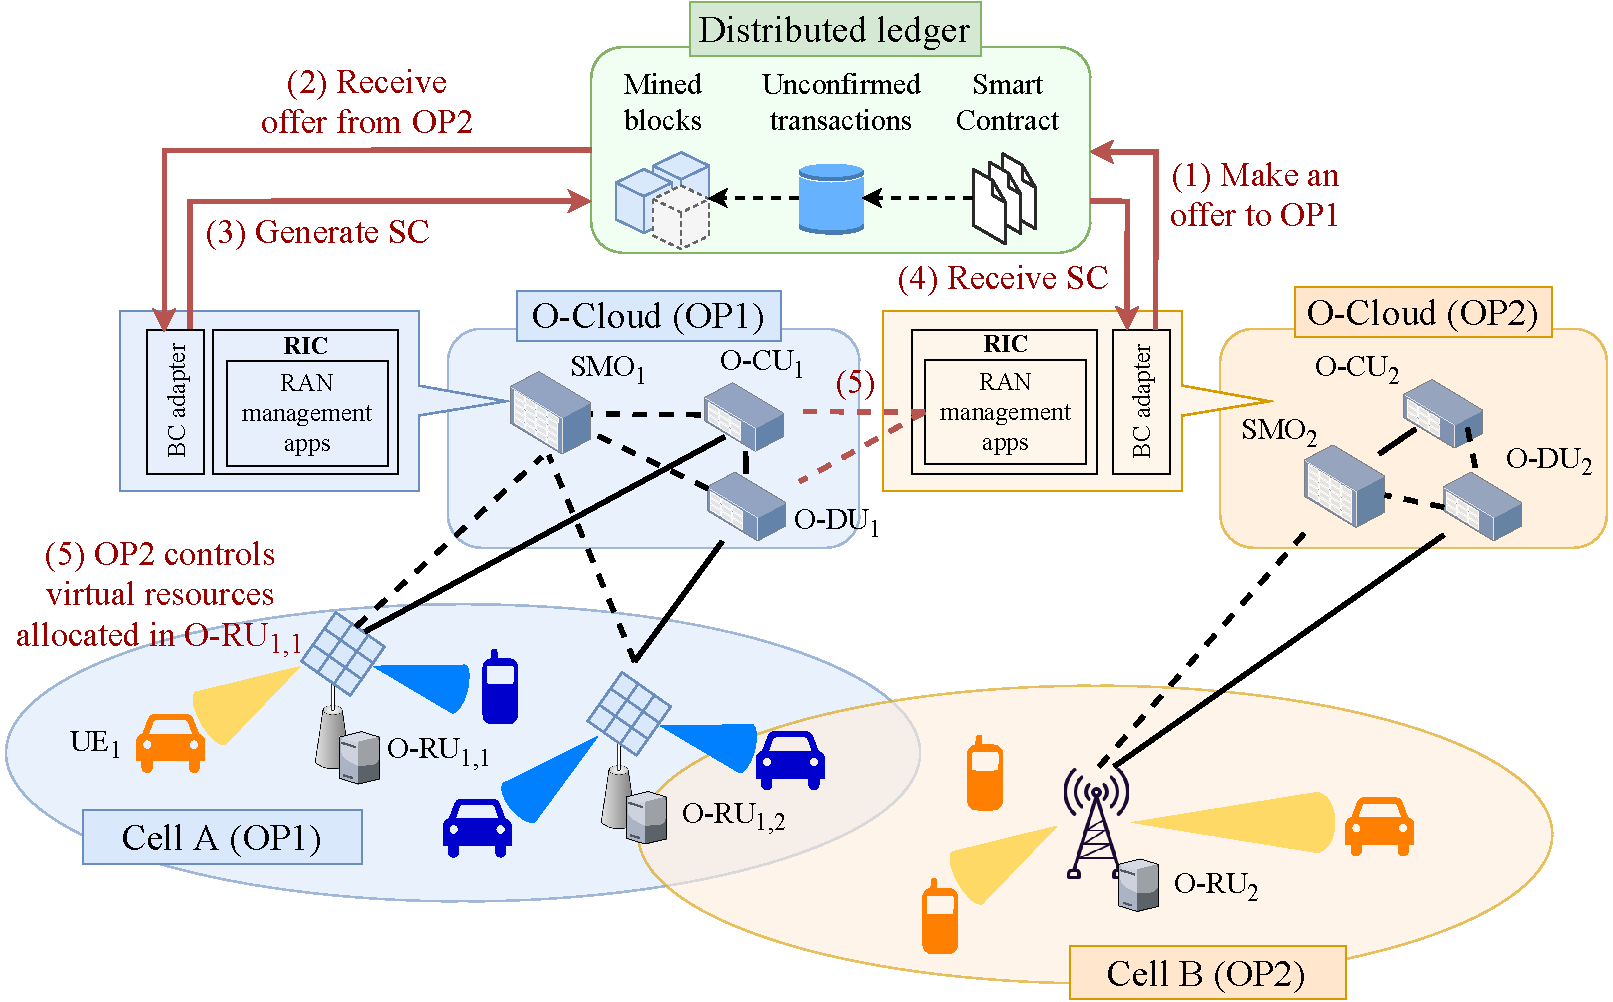
\includegraphics[width=\linewidth]{blockchain_ran-ecosystem}
\caption{BC-enabled RAN sharing ecosystem.}
\label{fig:blockchain_ecosystem}
\end{figure} 

The introduction of BC in network management has, however, also well-documented limitations (see \cite{FWilhelmi_PIMRC} and references therein). Maintaining a BC among a wide number of peers incurs heavy costs in computation, power, energy consumption, and memory usage. Running a BC in a mobile network represents a high traffic overhead due to the distribution of blocks across BC participants. The additional delay is another aspect that affects the network performance, the users' perception of the service, and the stability of the BC itself.%, due to vulnerability to forks.

The target of this paper is to first propose a BC-enabled O-RAN-based architecture for 6G, and then to evaluate some advantages and disadvantages incurred by the introduction of the BC in O-RAN management. Evaluation is done in terms of delay and overhead for service establishment as a function of the number of participating operators and BC parameters. The rest of this paper is organized as follows: Section~\ref{section:related_work} introduces the concept of BC technology and briefly overviews its standardization and application to network management. Section~\ref{section:architecture} describes the proposed architectural framework for O-RAN. The benefits and challenges of the proposal are discussed in Section~\ref{section:results}. Section~\ref{section:conclusions} concludes the paper.

%%%%%%%%%%%%%%%%%%%%%%%%%%%%
%% TUTORIAL SECTION ON BC AND NETWORK/RAN SHARING
%%%%%%%%%%%%%%%%%%%%%%%%%%%%
\section{A Primer on BC-enabled Network/RAN Sharing in cellular networks}
\label{section:related_work}

A BC is a type of distributed ledger technology (DLT) compiling transactions in blocks that are sequentially and cryptographically chained one after the other. A peer-to-peer (P2P)  network is in charge of maintaining the transactions' record on the BC. The miners organize the unconfirmed transactions into blocks and append them to the BC after achieving consensus. The consensus mechanism is an advanced cryptographic technique executed by all the participants of the BC, which allows validating the new block without the need to rely on a central trusted authority. BC was firstly introduced with the cryptocurrency Bitcoin. Successively, with the introduction of SCs, i.e., computer programs that run on top of the BC and self-execute the terms of a contract when specific conditions are met, BC's applications started appearing in multiple domains.%~\cite{cai2018decentralized}. 

On the one hand, the advent of BC raises issues related to memory usage, overhead, power consumption, and latency. These aspects require to be optimized by the BC protocol itself, besides interoperability issues, both at a technical level (how various interfaces talk to each other) and at a semantic level (how information exchanged is understood by the parties involved), which needs to be addressed by standardization activities. In this regard, important standardization organizations such as the International Telecommunication Union (ITU) and the European Telecommunications Standards Institute (ETSI) have been working on BC technology and released important documents concerning BC terminology, use cases, ecosystem, or architectural aspects (see, e.g.,~\cite{ITU1400,etsi2020permissioned}). Other initiatives like the European Blockchain Observatory and Forum, an open project to accelerate BC innovation within the EU, or the standardization of some DLT properties by W3C or Open Timestamps are also active. To obtain a broader view on the standardization of BC, we refer the interested reader to~\cite{konig2020comparing}.

On the other hand, the offered automation and trustworthiness of transactions are among the most valuable features of BC for trading in future mobile networks. In telecommunications, much research work has been ongoing in the area of BC-based Internet of Things (IoT) and beyond 5G (B5G)~\cite{nguyen2020blockchain}. BC has been widely envisioned to manage network sharing and trading of network slices for vertical applications~\cite{xu2020blockchain}. In particular, BC may become the basis of a decentralized and transparent platform for multi-party negotiation between the increasing number of stakeholders (e.g., VNF providers, multiple administrative domains) offering an end-to-end network slice. Recent architectural evolutions proposed by O-RAN~\cite{ORAN} already account for the RAN sharing use case, where multiple OPs are enabled to share their O-RAN infrastructure, while they are allowed to remotely configure and control the shared resources via remote, open, and newly standardized interfaces.   

In this paper, we focus on RAN sharing, and we advocate that the introduction of BC technologies can automate, accelerate, and secure the definition of the relationship with a well-defined SLA for the trade of resources. Previously, the authors of~\cite{xu2021ran} introduced an O-RAN-based architecture to conduct zero-trust mutual authentication over the unique BC-enabled routers, and switch functions with the identification exchanged over the BC. The main novelty proposed by~\cite{xu2021ran} is to introduce BC to decentralize RAN security aspects, in contrast to the current centralized solutions based on authentication and third-party trust. Additionally, other contributions target the vision of BC to facilitate resource trading in the RAN segment. In~\cite{maksymyuk2020blockchain}, the authors proposed a protocol for BC-based spectrum trading in 5G/6G networks. Finally, the work in~\cite{togou2020dbns} described an architecture that facilitates the dynamic leasing of resources among network operators to support cross-domain services. The cornerstone of this architecture is a brokering layer that relies on a BC-based bidding system to exchange resources.

%%%%%%%%%%%%%%%%%%%%%%%%%%%%
%% ARCHITECTURE
%%%%%%%%%%%%%%%%%%%%%%%%%%%%
\section{Architectural Framework for BC-enabled RAN Sharing}
\label{section:architecture}
In this section, we study how RAN sharing as enabled by the O-RAN architecture can be improved to become dynamic and autonomous through BC. We first introduce the basics of O-RAN and then discuss the role of the proposed new blocks.

\subsection{O-RAN Architecture}
The O-RAN Alliance was born in February 2018 to continue the evolution of 3GPP RAN architecture in areas like non-public networks, self-organized networks, and integrated access and backhaul. Its major tenant is to define open interfaces between elements implemented in general-purpose hardware. It is the first standard to enable multi-vendor RAN, and RAN virtualization, thus favoring efficient splits over the protocol stack for network slicing purposes. This flexibility allows to bring in new radio players and gives plenty of opportunities to operators to optimize deployments for specific performance requirements at a much better cost. 

\begin{figure*}[ht!]    
\centering
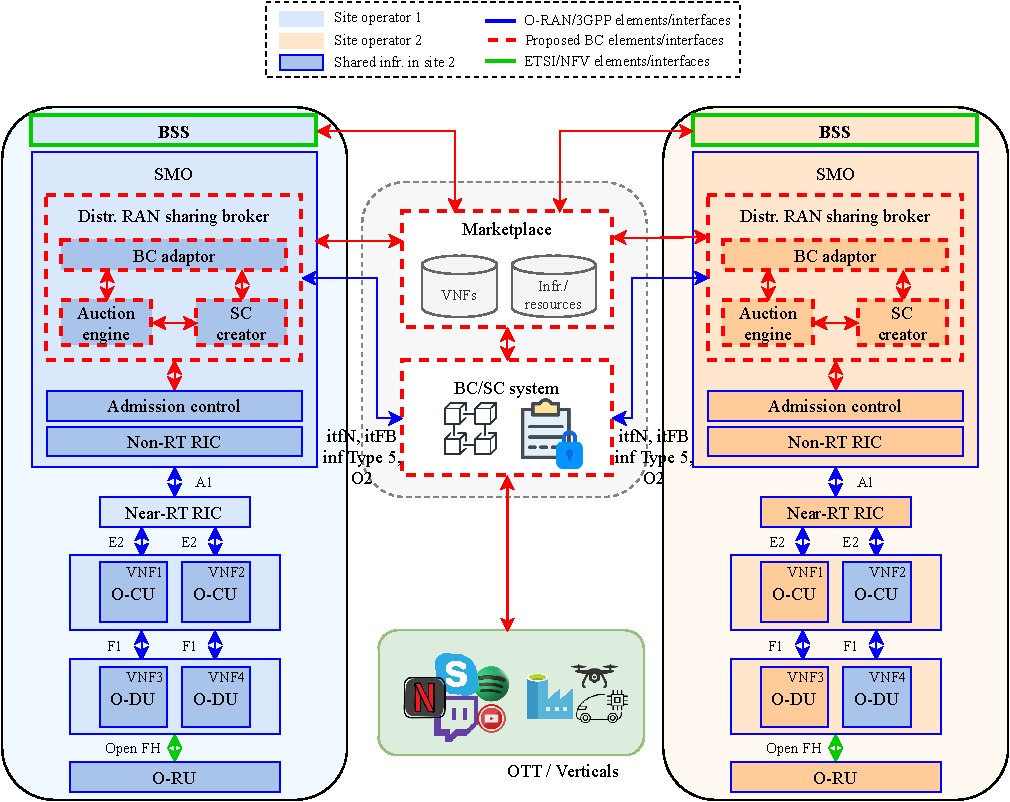
\includegraphics[width=0.75\textwidth]{functionalarchitecture2.pdf}
\caption{Functional BC-enabled O-RAN architecture.}
\label{fig:functionalarchitecture}
\end{figure*}

The O-RAN architecture, based on the original 3GPP proposal in TS 38.401, is shown in Fig.~\ref{fig:functionalarchitecture} for two operators sharing a coverage area. Specifically, the figure represents a RAN sharing-compliant O-RAN architecture that allows operators to remotely configure the shared network resources independently from configuration and operating strategies of the hosting operator. This RAN sharing use case is extensible to MVNOs, service providers, and verticals requesting RAN resources. The main O-RAN modules (marked in blue), deployed as VNFs or containers, and whose interfaces are defined by O-RAN in~\cite{ORAN2}, are as follows: 
\begin{itemize}
    \item \textbf{System management and orchestration (SMO):} The SMO, similar to other architectures based on ETSI NFV's, provides a variety of network management functionalities. In the context of O-RAN and for what concerns the RAN functionalities, it oversees all the orchestration, management, and automation aspects. It includes fault, configuration, accounting, performance, security (FCAPS) support for O-RAN functions, such as installation, configuration, or performance, fault, and file management. In addition, it includes the newly introduced non-real-time (non-RT) Radio Intelligent Controller (RIC) for intelligent RAN optimization. These functionalities are supported by newly introduced interfaces such as A1, O1, and O2.
    %
    \item \textbf{O-RAN centralized unit (O-CU):} The O-CU hosts the gNB protocols of Radio Resource Control (RRC), Service Data Adaptation Protocol (SDAP), and Packet Data Convergence Protocol (PDCP), and is connected to the O-DU via F1-C and F1-U interfaces, for control and data planes, respectively. The O-CU controls the operation of multiple O-DU over midhaul interfaces. The split architecture enables different distributions of protocol stack between O-CU and O-DU, depending on the midhaul availability and the network design.
    %
    \item \textbf{O-RAN decentralized unit (O-DU):} The O-DU hosts the radio link control (RLC), the medium access control (MAC), and PHY-high layers of the gNB, and is connected to the O-RU via the Open Fronthaul interface. This node includes a subset of the eNB/gNB functions, depending on the functional split option, and its operation is controlled by the O-CU.
    %
    \item \textbf{Radio intelligent controller (RIC):} O-CUs are controlled by the non-RT and the near-RT RIC modules, supporting tasks with more or less than one~second latency, respectively. Through these modules, the {O-RAN} architecture strives the industry to introduce embedded artificial intelligence (AI) in the system. RICs are based on software apps to orchestrate and manage the RAN. Applications like mobility management, admission control, and interference management are available as apps on the RIC, which enforces network policies to the radio segment. Non-RT RIC is implemented inside the SMO and includes service and policy management, RAN analytics, and model training for the near-RT RIC. The trained model is managed by the SMO for deployment and received by the near-RT RIC through A1 interface. The near-RT RIC uses the E2 interface to collect information at UE and cell basis and perform self-optimization tasks across the heterogeneous RAN (e.g., formed by macros, massive MIMO, small cells).
\end{itemize}
O-RAN has studied different options for CU/DU/RU deployment, including location in regional clouds, or operator-specific sites. The so-called \textit{Scenario B} is the initial priority of {O-RAN}, where O-CU and O-DU are located together in a cloud, while the O-RU is located in a proprietary cell site.

\subsection{BC-enabled O-RAN}
We propose to enrich the O-RAN architecture with new functional blocks for automatic, dynamic sharing of RAN resources through BC. The functional architecture is depicted in Fig.~\ref{fig:functionalarchitecture}, where the newly proposed modules are in red. The introduction of BC can automate, accelerate and secure the RAN sharing start-up phase between OP$_i$ and OP$_j$ to define the relationship with SLAs for resource trading. Specifically, OP$_i$ makes its {O-RAN} infrastructure available and hosts the virtual RAN functions of a second OP$_j$. Remote configuration and monitoring of instantiated VNFs in the host infrastructure of OP$_i$ is allowed through O1, O2, and E2 interfaces. Performance monitoring is implemented during the running phase and complemented by AI functionalities offered by RIC modules, to ensure SLA enforcement. 

The proposed architecture includes different additions to the O-RAN baseline, like the Business Support System (BSS), inherited from ETSI-NFV architecture, for the operator to deliver product, customer, and revenue management (billing). The SMO, besides the already introduced non-RT RIC, includes the admission control functionality that decides whether new VNFs can be leased on the site infrastructure. This information is fed to the newly introduced \textit{distributed RAN sharing broker}. In addition, we propose a \textit{marketplace} where OPs can opt to advertise the infrastructure they are willing to offer, a \textit{BC/SC system}, and the following set of new interfaces: 
\begin{itemize}
    \item An SMO internal interface between the admission control and the RAN sharing broker.
    \item Different broker internal interfaces across its elements.
    \item An interface between the BSS and the BC/SC system.
    \item An interface between the SMO and the BC/SC system (Itf-BC), which can be newly defined or can reuse already available interfaces proposed by O-RAN and 3GPP (i.e., O2, Itf-N, Itf-B, and Type~5 interface).
    \item Vertical industries and OTT providers may also interact with the BC and the OPs providing infrastructure through the so-called Service Capability Exposure Function (SCEF).
\end{itemize}

The distributed \textit{RAN sharing broker} is the entity that manages and offers RAN VNFs. The concept of broker has been previously introduced in~\cite{samdanis2016network} for network slicing, as a management point to gather requests from multiple parties such as MVNOs, OTTs, or vertical providers, and to perform admission control. The blocks included in the distributed RAN sharing broker are:
\begin{itemize}
    \item \textbf{SC creator}: The SC creator is in charge of mapping requirements and preferences into an SC format so that other operators are informed about the selected service from a marketplace, or about information to participate in an auction. The SC defines the SLA that needs to be monitored during the running phase, including information such as the resources type, required QoS, service duration, or tolerance indicators. Once the SC is compiled and distributed, the auction engine is triggered (where applicable).
    \item \textbf{Auction engine}: It is in charge of handling the auction process. For the requesting OP, the auction engine is responsible of collecting the bids submitted by the OPs participating in the auction, selecting the winner based on a precise algorithm for end users' expected satisfaction, and triggering the communication between the own SMO and the SMO of the selected OP to instantiate the requested VNFs. The auction starts after deploying the SC, and is concluded after a predefined period depending on time, reception of a certain number of bids, achievement of a price target, etc. For candidate OPs, the auction engine defines the bid to be submitted based on internal bid algorithms depending on business variables, available resources, the price for a unit of resources, special discounts, and expected return of investment. During each auction process, bids and decisions are securely recorded inside the BC for distributed decisions related to auctions and future audits.
    \item \textbf{BC adaptor}: The BC adaptor is the entity in charge of handling the communication with the BC and registering the OP to it.
\end{itemize}

The BC in the proposed architecture is private, so only operators deploying a RAN sharing broker can join it. We propose two different mechanisms to exchange RAN resources within the proposed architecture (see Fig.~\ref{fig:functionalarchitectureflowdiagram}):
\begin{itemize}
    \item \textbf{Marketplace-oriented}: All OPs with VNFs, infrastructure, and resources to offer, advertise them with specific prices in a catalog (i.e., marketplace), where other stakeholders select the desired service. To participate in the marketplace, the OP registers the information of interest (e.g., available resources, prices) in the BC. In the flow diagram, OP$_j$ is interested in leasing a VNF from another OP, so it accesses the marketplace to acquire one. After selecting a sharing provider OP$_i$, the SC creator in the RAN sharing broker of OP$_j$ prepares an SC defining the SLA, based on the offer identified in the marketplace. This is distributed in the BC and received by the BC adaptor of OP$_i$, which translates the SC into requirements and sends them to the admission control of the SMO for evaluation. If the request is accepted, a VNF is instantiated in OP$_i$'s infrastructure to be remotely configured (during the configuration phase) by OP$_j$ through the open interfaces defined in O-RAN (O1/O2 remote). During the running phase, the SLA is monitored through RICs at OP$_j$ site. Monitoring support from the hosted VNFs, with radio state reports, is realized through the O-RAN native E2-remote interface. Service updates are sent to the RAN sharing broker so that the SC creator prepares a new SC, which is then registered in the BC and analyzed by OP$_i$'s admission control.
    %
    \item \textbf{Auction-oriented}: In this variant of the procedure, the serving OP$_i$ is selected using an auction procedure, which is expected to better fit the offer of service and provide a more efficient resource usage. The OP$_j$ interested in leasing resources from another OP defines the requirements and desired price for the needed resources and sends them to the SC creator of the RAN sharing broker of OP$_j$. The SC creator prepares an SC, which is distributed through the BC. Other OPs interested in offering to lease their resources, evaluate availability through admission control functionality, and if the resources are available, participate in the auction submitting a bid through their auction engine. The auction engines distribute the bids from the candidate OPs through the BC. OP$_j$'s auction engine collects the bids and decides the target OP$_i$ to host the desired VNFs. From this moment, the procedure is similar to the marketplace case. The provisioning request is sent to the hosting OP, to the RAN sharing broker, and an instantiation request is sent to the orchestrator to be instantiated in the platform of  OP$_i$ site. 
\end{itemize}

\begin{figure}[ht!]
\centering
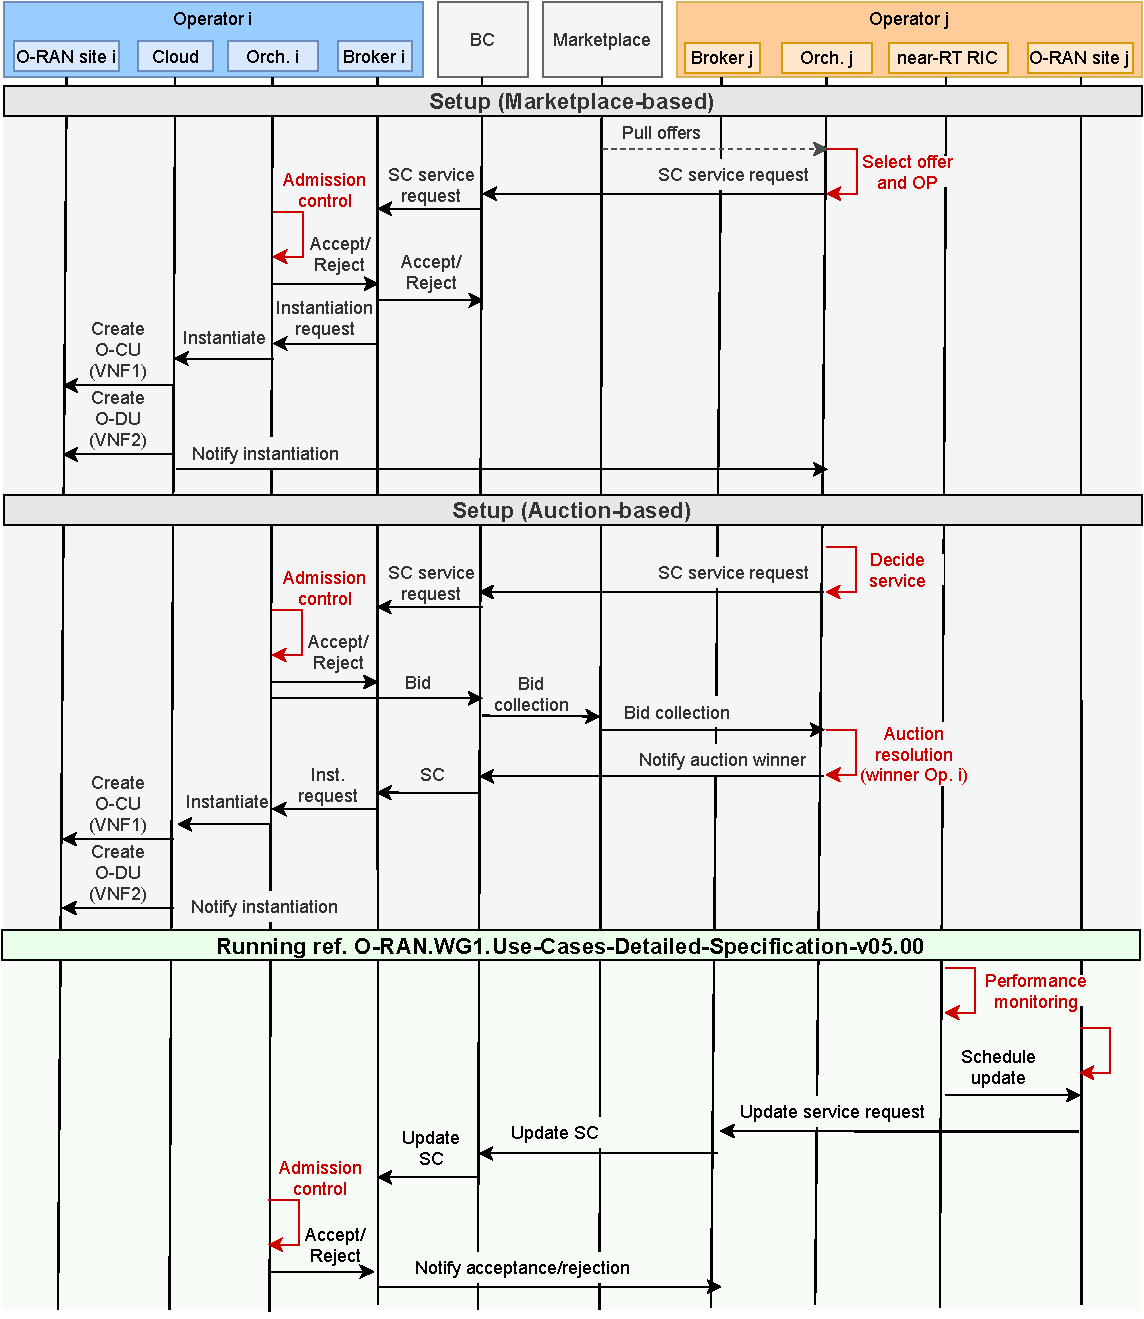
\includegraphics[width=1\columnwidth]{flowdiagram_complete.pdf}
\caption{Flow diagram of the BC-enabled O-RAN functional architecture, for marketplace and auction-oriented cases.}
\label{fig:functionalarchitectureflowdiagram}
\end{figure}

%%%%%%%%%%%%%%%%%%%%%%%%%%%%
%% USE CASE
%%%%%%%%%%%%%%%%%%%%%%%%%%%%
\section{BC-enabled RAN sharing: opportunities and challenges}
\label{section:results}
The introduction of BC-enabled RAN sharing offers OPs new opportunities for new revenue incomes by capitalizing on available infrastructure. In this section, we analyze the different opportunities and challenges, as well as the trade-offs among them, of the proposed BC-enabled RAN sharing architectural framework. The most important opportunities offered by BC and SC to traditional RAN sharing are:
\begin{enumerate}
    \item \textbf{Automated management:} By removing long interactions with third parties in the negotiation for sharing resources, improved network management efficiency is expected.
    %
    \item \textbf{Resources efficiency:} Through automated RAN sharing, resources can be fully harnessed by multiple parties, thus leading to higher network capacity, more coverage, and, consequently, improved users' satisfaction.
    %
    \item \textbf{Competitiveness:} With the entry of new actors to the RAN sharing ecosystem, competitiveness is expected to be boosted, which leads to further service diversification and additional possibilities to improve the network infrastructure. This is expected to attract more investments in the network.
    %
    \item \textbf{Auditablity:} The traceability of every interaction in a BC allows for improved trust and transparency in RAN sharing. This is an important aspect to take into account, considering the recent issues raised by, e.g., Ericsson warning on O-RAN security~\cite{boswell2020security}.
\end{enumerate}

Concerning the challenges, BC/SC systems have several well-documented drawbacks to take into account when considering their inclusion in an established trading system: 
\begin{enumerate}
    \item \textbf{Communication overhead:} The communication among peer nodes and miners in BC generates overhead, which increases with the number of participants and the duration of the requested services (accurate short-term requests vs long-term fixed contracts).
    %
    \item \textbf{Transaction confirmation latency:} The distribution of transactions and blocks across the BC determines the delay for instantiating RAN functions in the infrastructure providers' platform. The transaction confirmation delay in a BC strongly depends on the adopted consensus mechanism and other parameters like the mining difficulty. A detailed model to estimate the transaction confirmation latency based on those parameters in wireless blockchain networks can be found in~\cite{FWilhelmi_PIMRC}.
    %
    \item \textbf{Stability:} The stability of a BC is strongly related to the network consensus. In this regard, forks may threaten the BC stability. A fork is a split of a BC, which occurs when the difference in time between two nodes finding the nonce is lower than the time required by a node to distribute the winning block through the BC. As a result, the performance of a BC may be jeopardized by a low network capacity. Moreover, game-theoretical aspects may motivate selfish behaviors among miners (e.g., releasing a block at the appropriate time to gain an advantage), thus adding instability to the BC. %Forks may incur additional transaction confirmation delay. 
    %
    \item \textbf{Scalability:} Given the nature of BC, whereby all the transactions need to be propagated and stored, an increase in the number of BC users and transactions can represent both a communication and a storage issue. Besides, BC is originally limited by the block size and the mining difficulty (see, e.g., the case of Bitcoin), which limits the effective transactions rate. 
\end{enumerate}

Fig.~\ref{fig:performance} compares performance in terms of capacity, satisfaction, and efficiency for \textit{(i)} static scenario where RAN sharing is not enabled, \textit{(ii)} marketplace, and \textit{(iii)} auction-oriented approaches, in cellular random deployments with up to 19~cells and 200~users.\footnote{All the source code and background information of simulación results are openly available at \textit{\url{https://github.com/fwilhelmi/blockchain_enabled_ran_architecture}, accessed on Jul. 31, 2021}.} In particular, we compute (1) the user capacity (in Mbps), as a function of the set of resources allocated to each user and its signal to noise and interference ratio (SINR); (2) the user satisfaction (between 0 and 1), as a function of the obtained service and the price paid for it~\cite{giupponi2008novel}; (3) the efficiency of each approach (as a ratio), by indicating the degree to which base station (BS) resources are appropriately assigned to users to meet their needs. %Specifically, the efficiency is computed as the inverse of the difference between the load requested by users and the actual load of the BSs.

\begin{figure}[ht!]
\centering
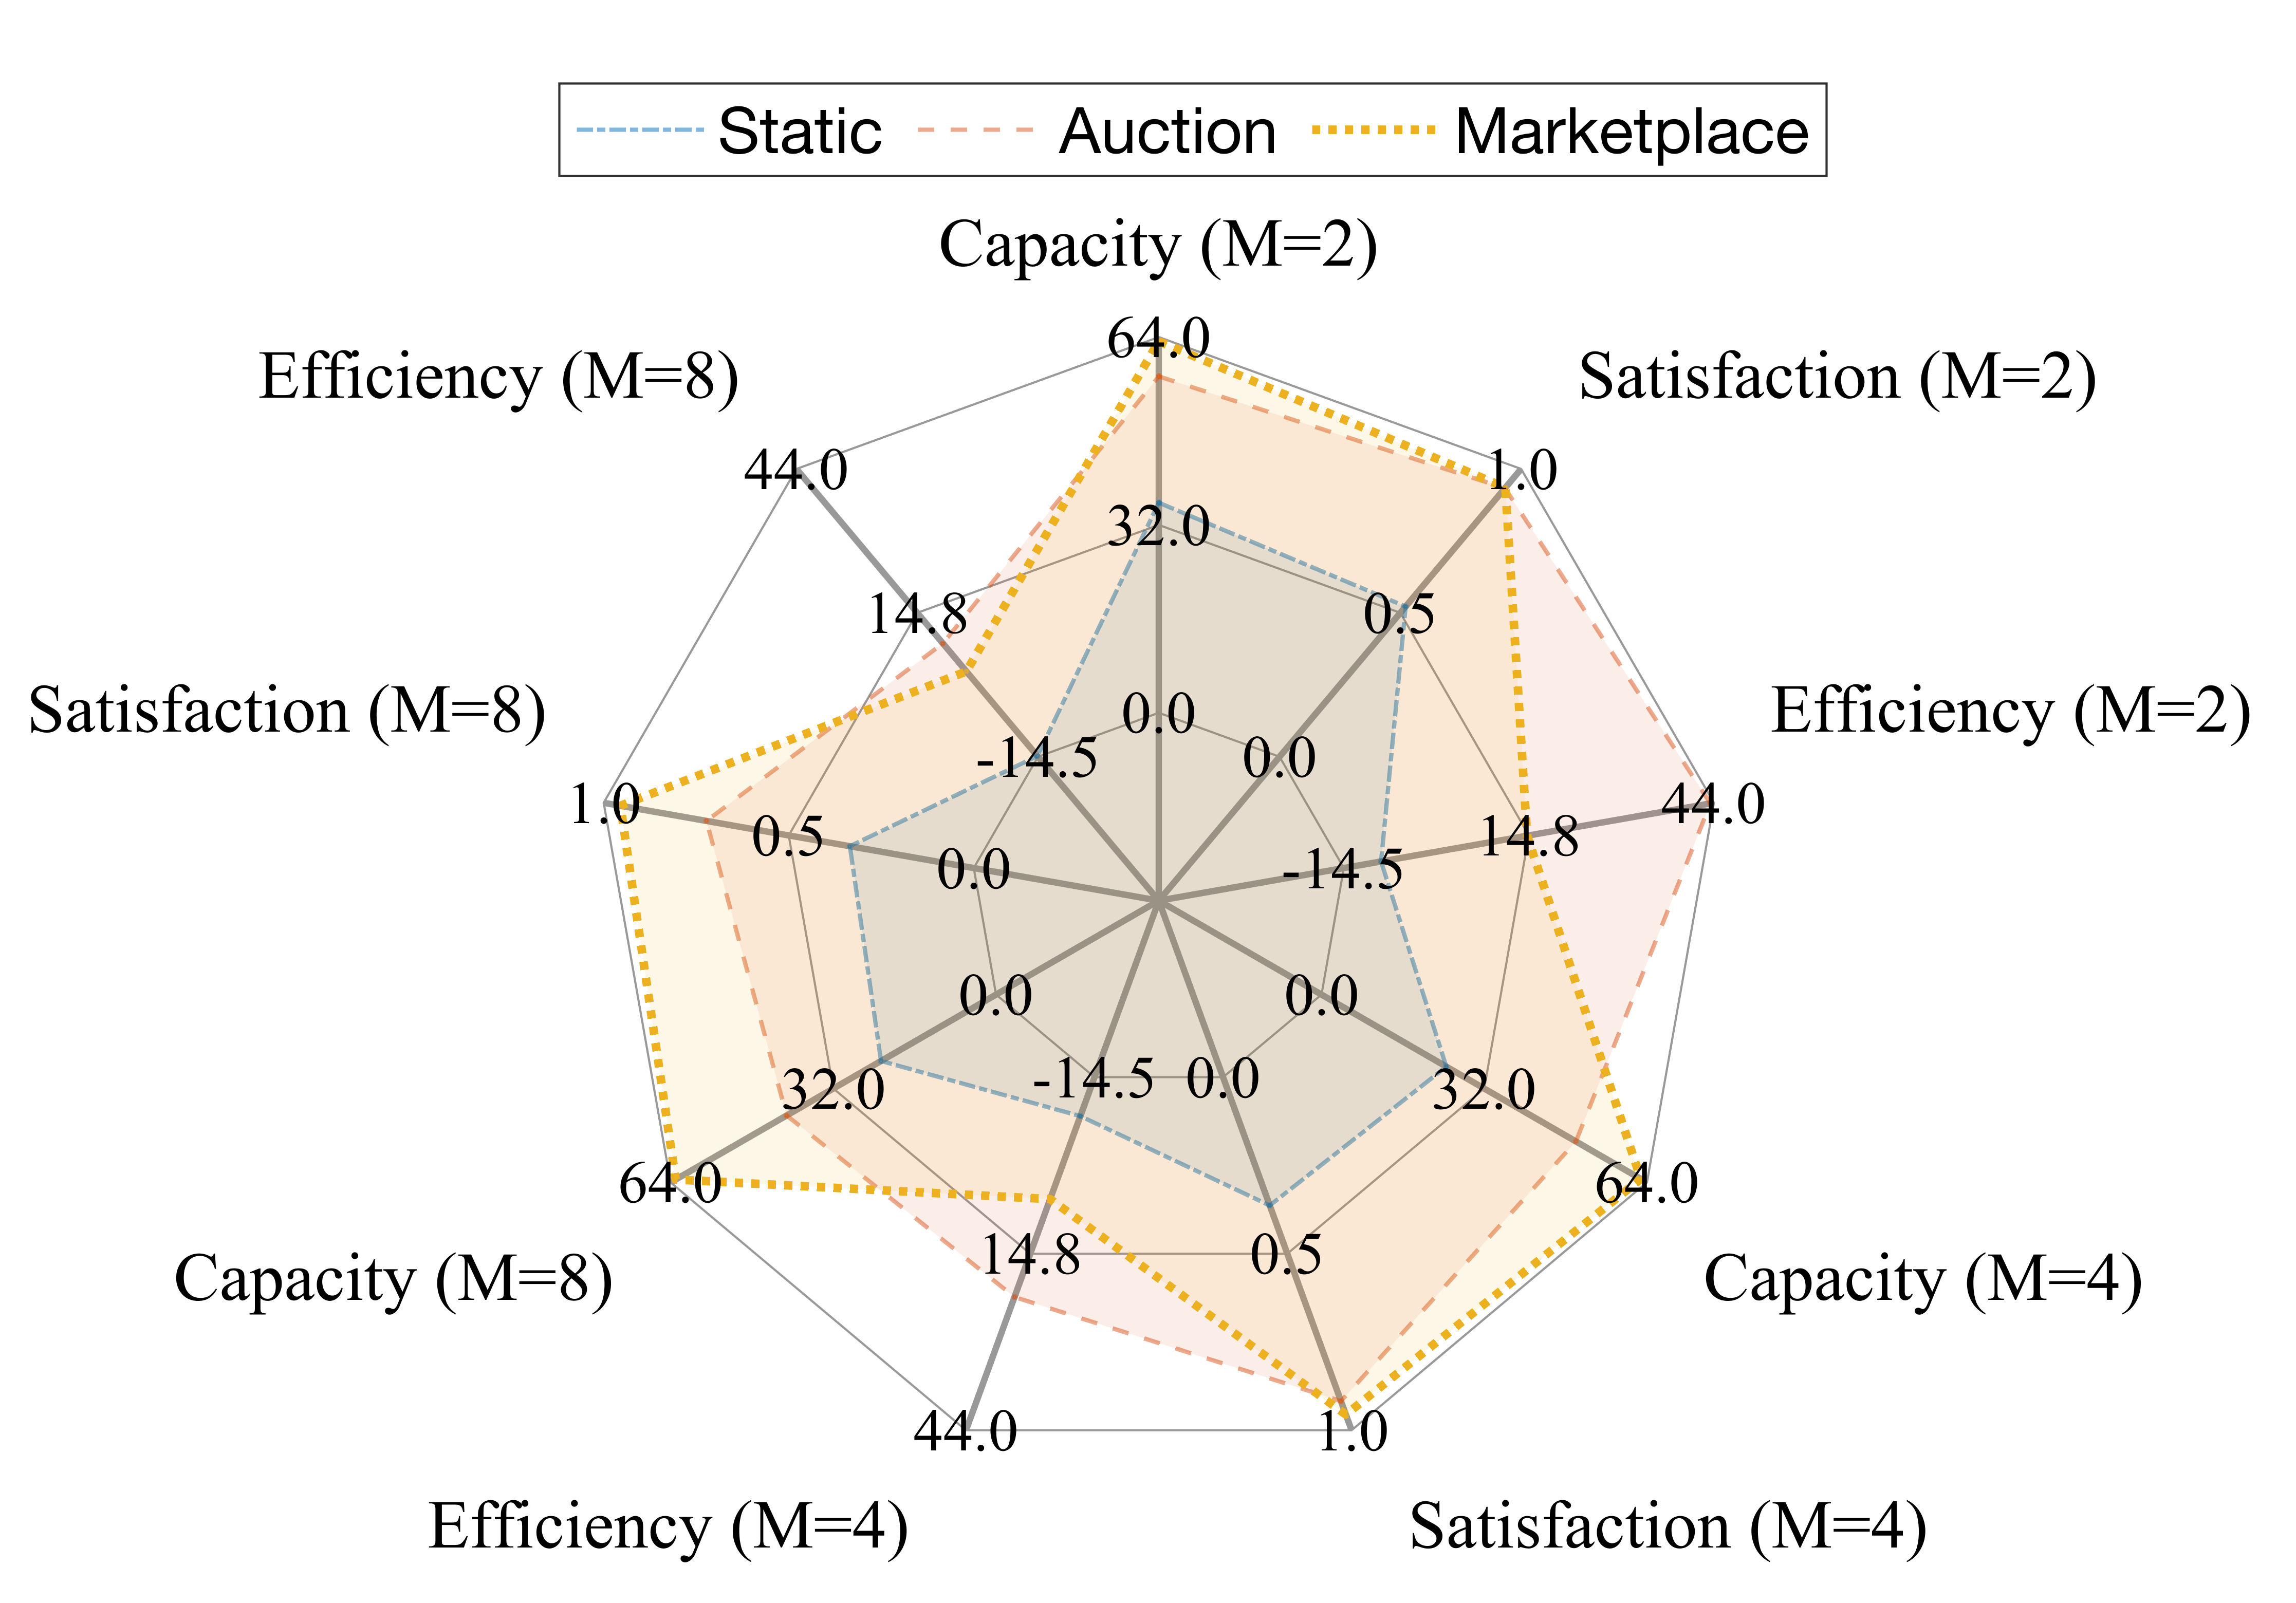
\includegraphics[width=.9\linewidth]{spiderplot.png}
\caption{UE performance and efficiency of the different BC-enabled RAN sharing mechansism compared to the static situation.}
\label{fig:performance}
\end{figure}

As shown in Fig.~\ref{fig:performance}, both BC-enabled auction and marketplace solutions outperform the static one, in terms of user's capacity and user's satisfaction. The automation of the exchange among OPs is essential to improve the utilization of the infrastructure, which ultimately leads to increased gains and profits of both sharing and leasing OPs. Moreover, the marketplace provides higher capacity and user satisfaction, since more resources than needed are allocated on average, based on pre-configured offers in the marketplace. Thus, new users can be served earlier with the spare capacity already available at the OP side. However, regarding efficiency, the auction approach outperforms the marketplace option, because the resources allocated to the users can be perfectly adjusted to their demands. In contrast, the marketplace offers a simpler allocation protocol, at the price of lower flexibility and less tailored service.

We now showcase trade-offs by focusing on the overhead and the additional delay incurred by the proposed BC-enabled RAN sharing solution. Notice that we consider the total time needed to define the SC with the agreed service and to distribute it through the BC. This delay is added to the baseline O-RAN delay between the service request and the instantiation of the VNF at a given operator's infrastructure site. In the marketplace case, the BC delay delay includes the time for propagating the SC service request and automatically enforcing it based on marketplace offers, whereas the auction-based procedure also includes the distribution of bids over the BC. Fig.~\ref{fig:delay} and Fig.~\ref{fig:overhead} illustrate the BC delay and overhead, respectively, associated to both auction and marketplace-based solutions. The results include different numbers of operators (2, 4, and 8), users' request rates (1, 5, and 10 service requests per second), and block size values (from 3,000 to 30,000 bits).

\begin{figure}[ht!]
\centering
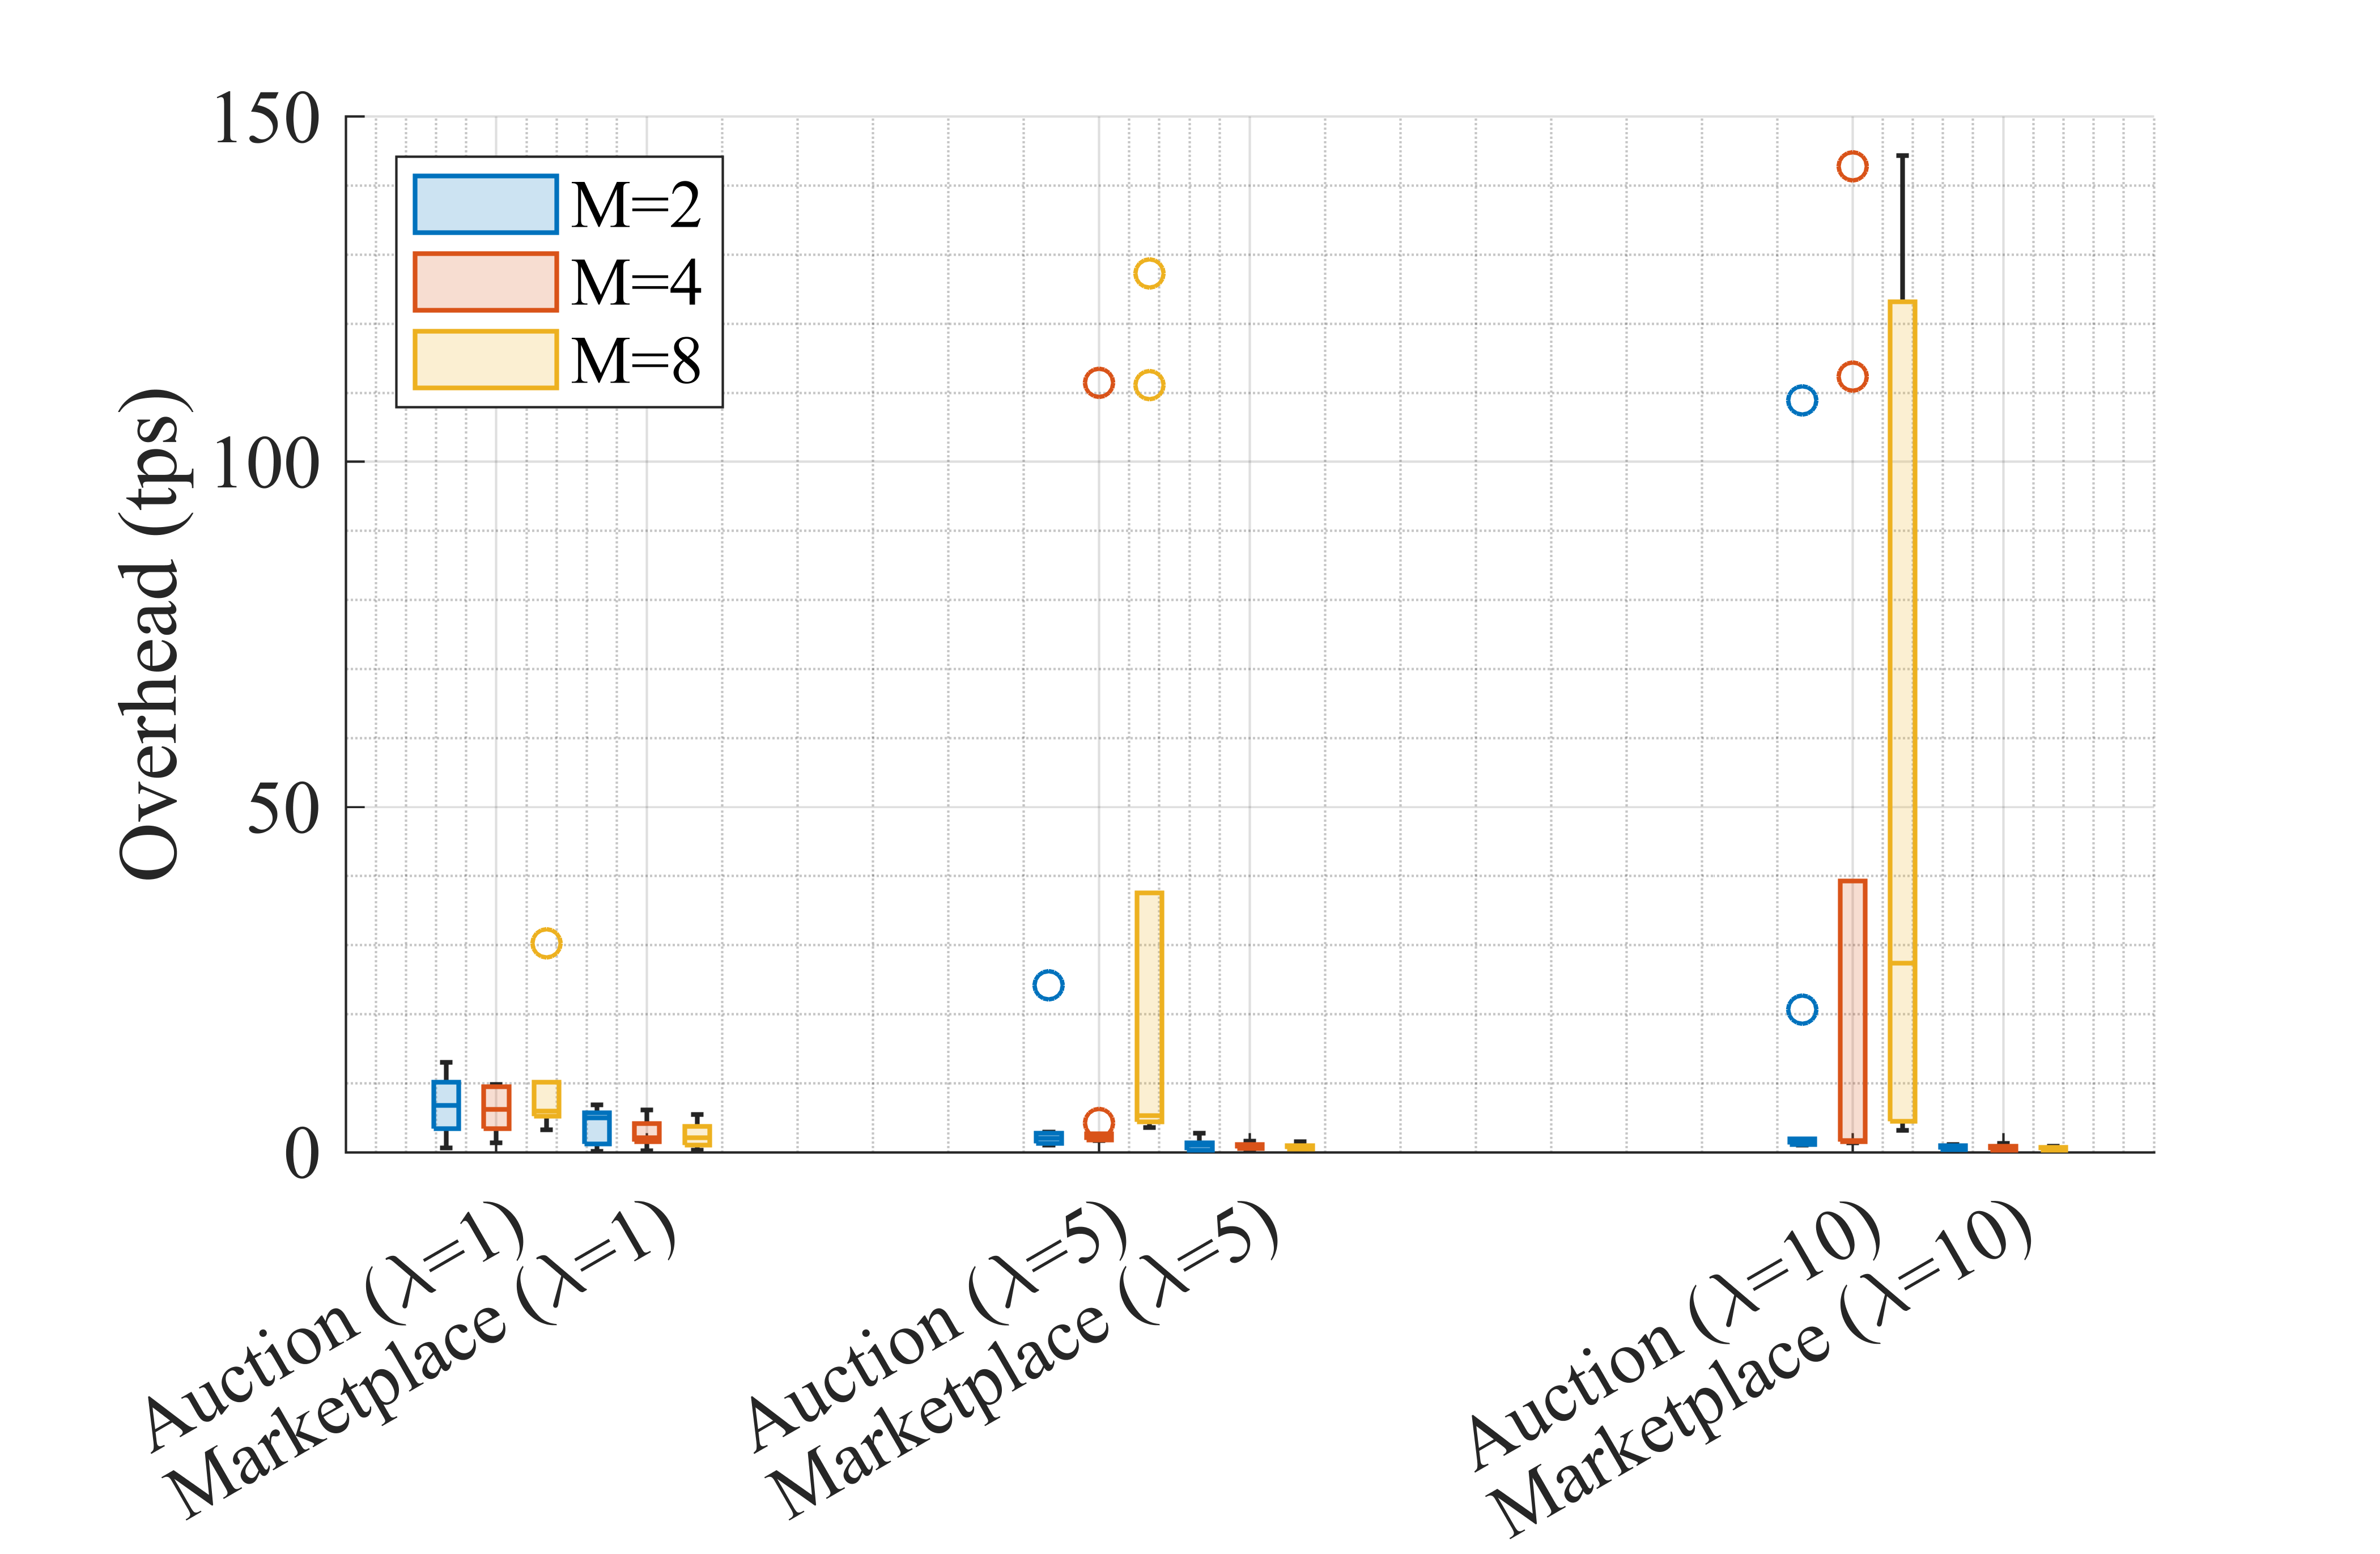
\includegraphics[width=.85\linewidth]{delay_new.png}
\caption{BC delay experienced by the auction and marketplace-oriented RAN sharing solutions.}%, different block sizes, user arrival rates, and number of operators.
\label{fig:delay}
\end{figure}

\begin{figure}[ht!]
\centering
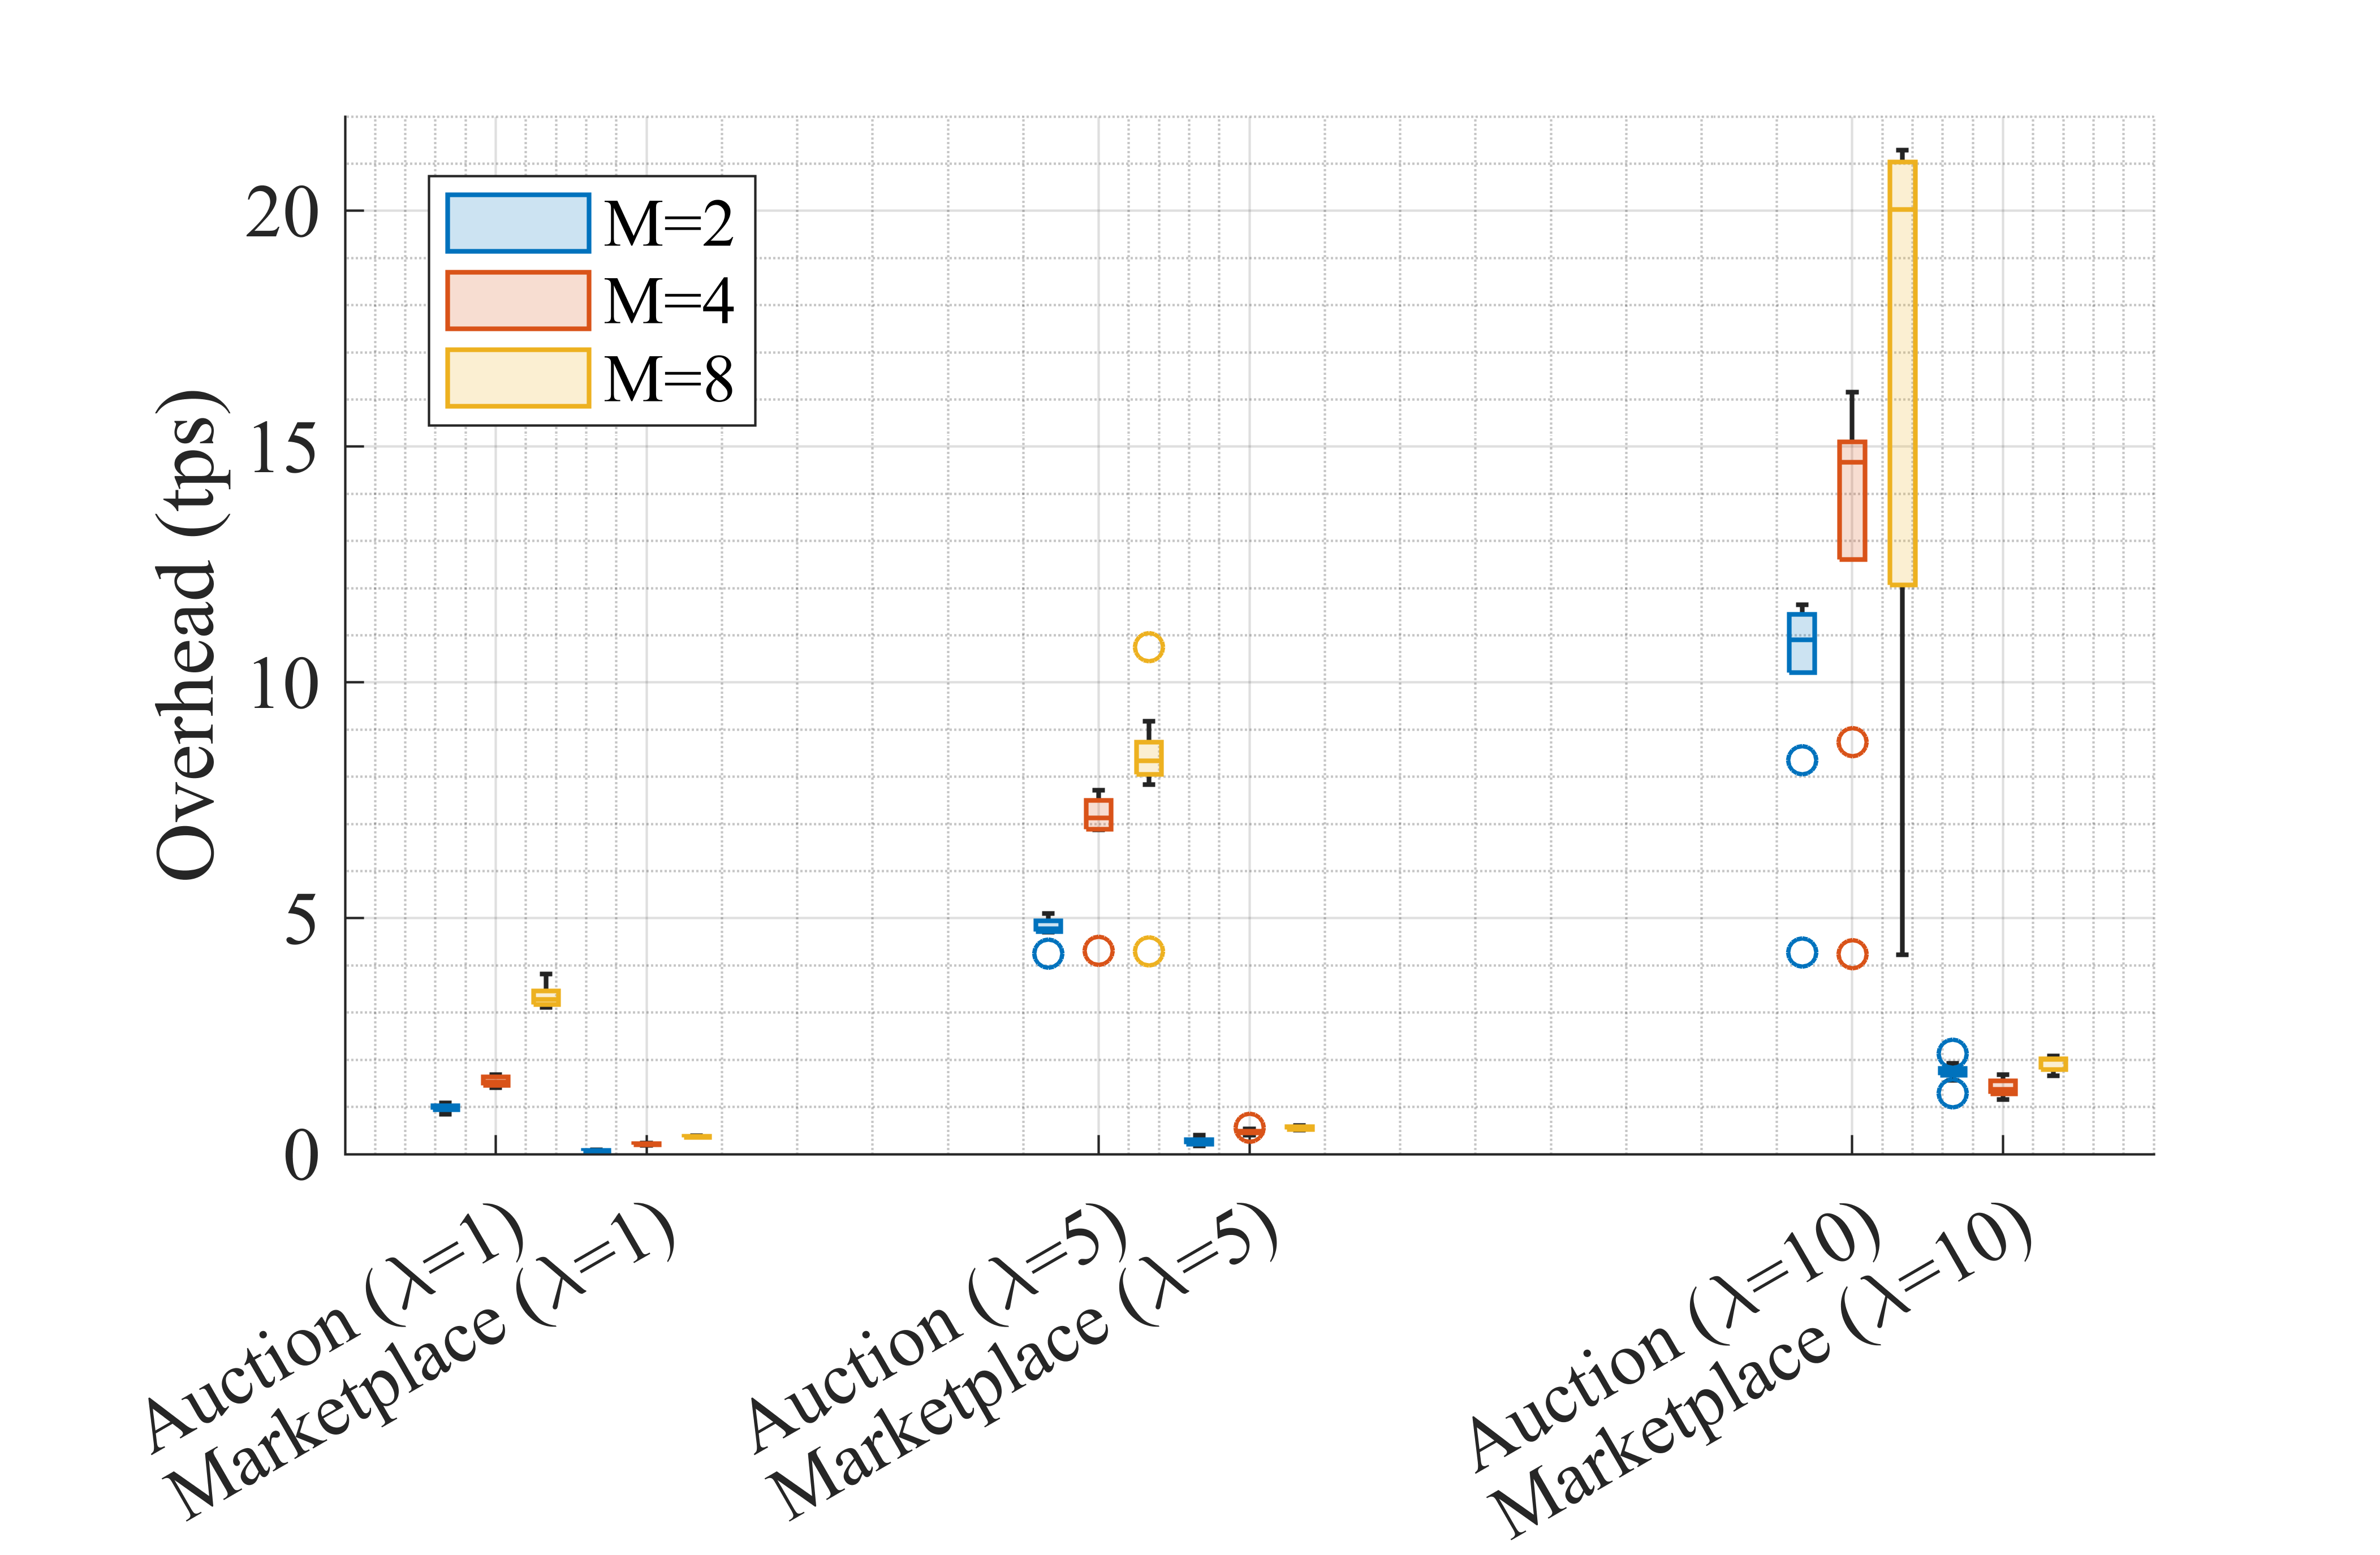
\includegraphics[width=.85\linewidth]{overhead_new.png}
\caption{BC overhead experienced by the auction and marketplace-oriented RAN sharing solutions.}
\label{fig:overhead}
\end{figure}

%\begin{figure}[ht!]
%\centering
%\subfigure[]{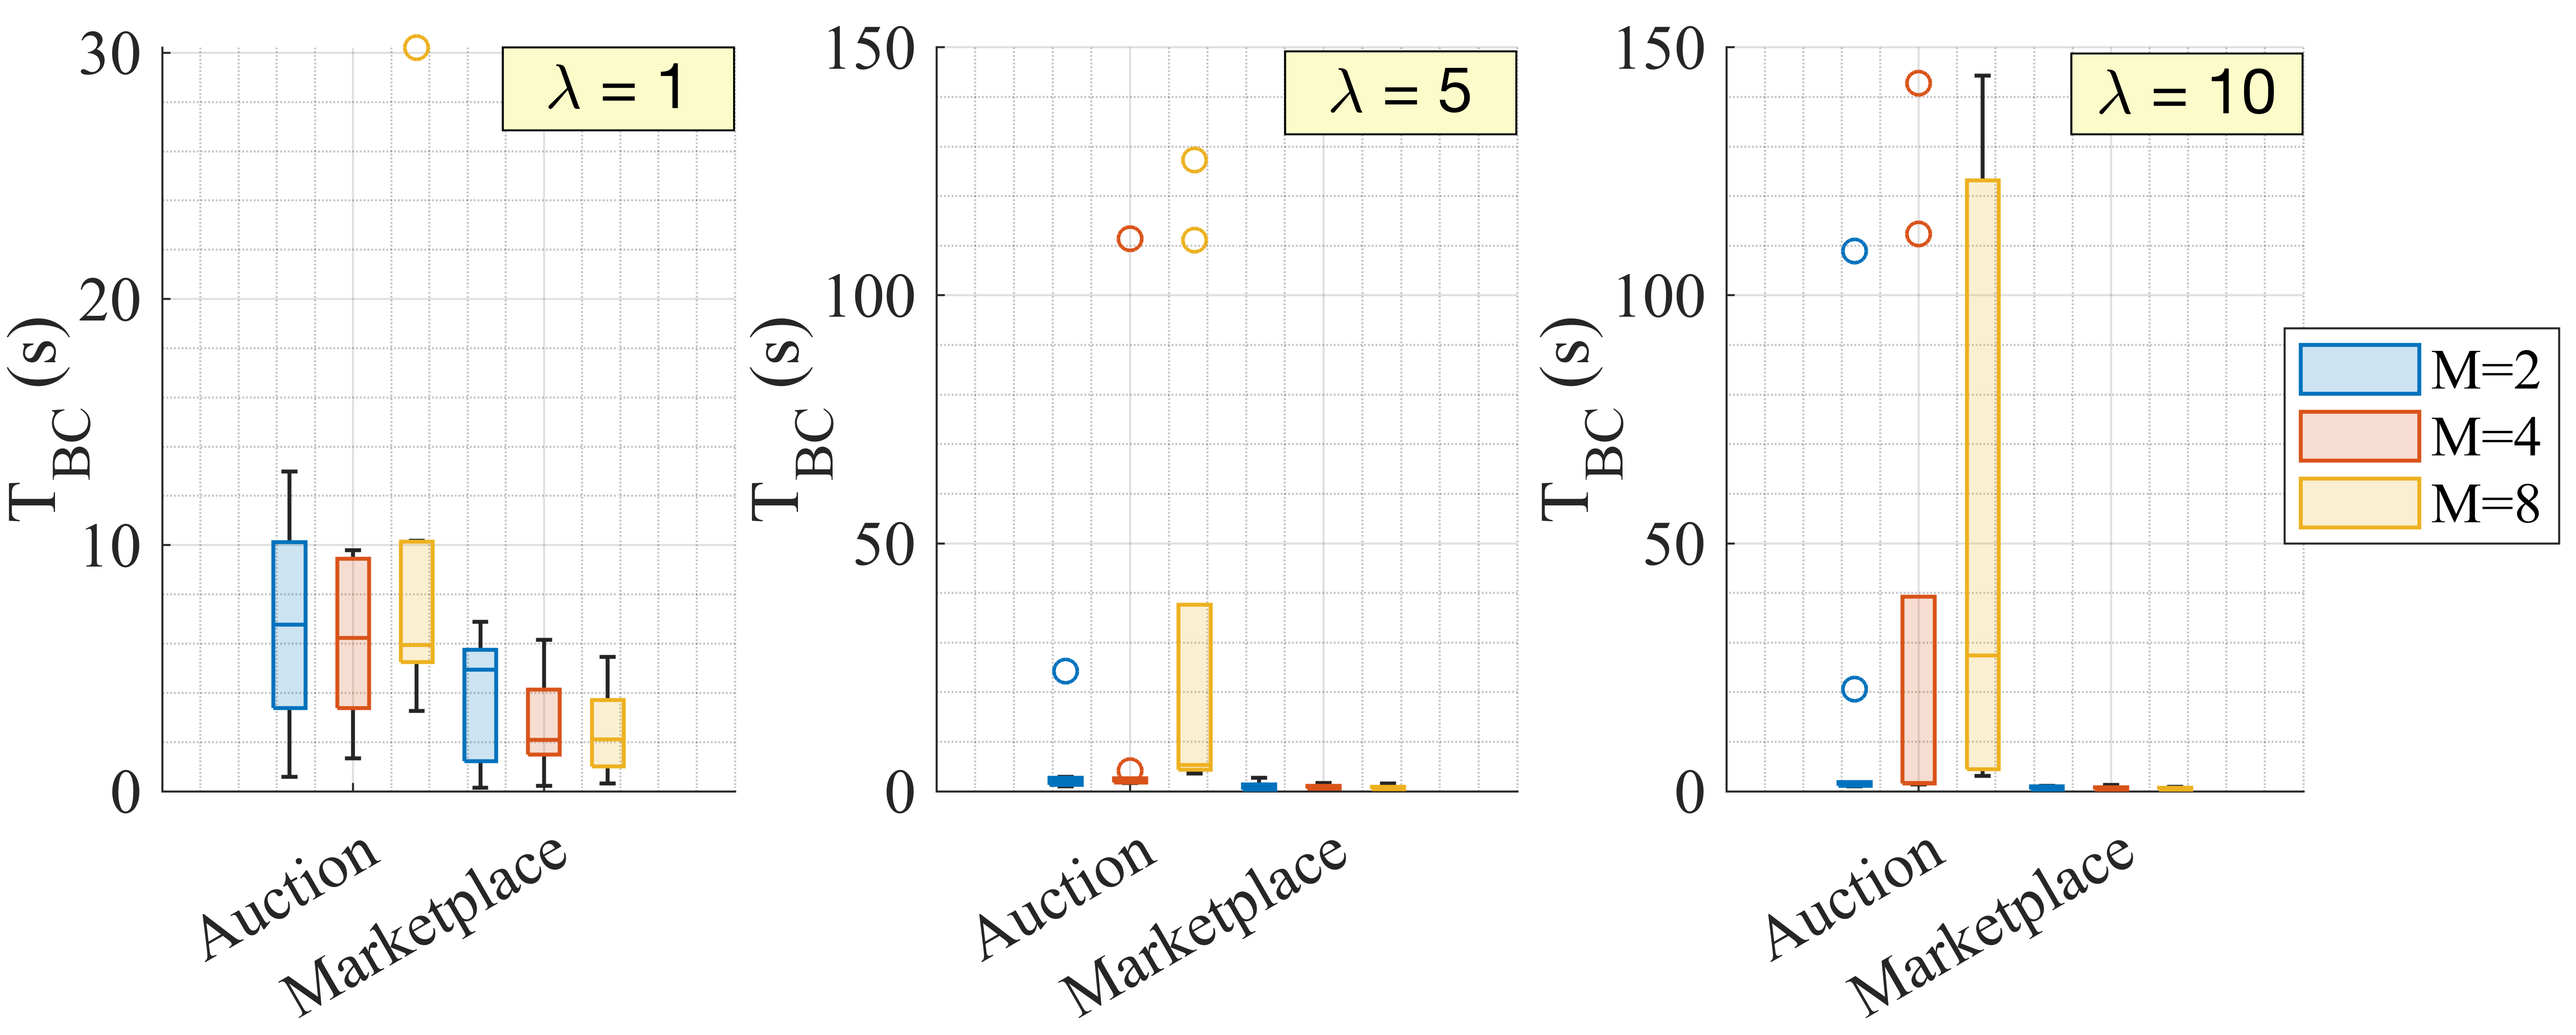
\includegraphics[width=\columnwidth]{boxplot_combined_delay.png}\label{fig:2}} 
%\subfigure[]{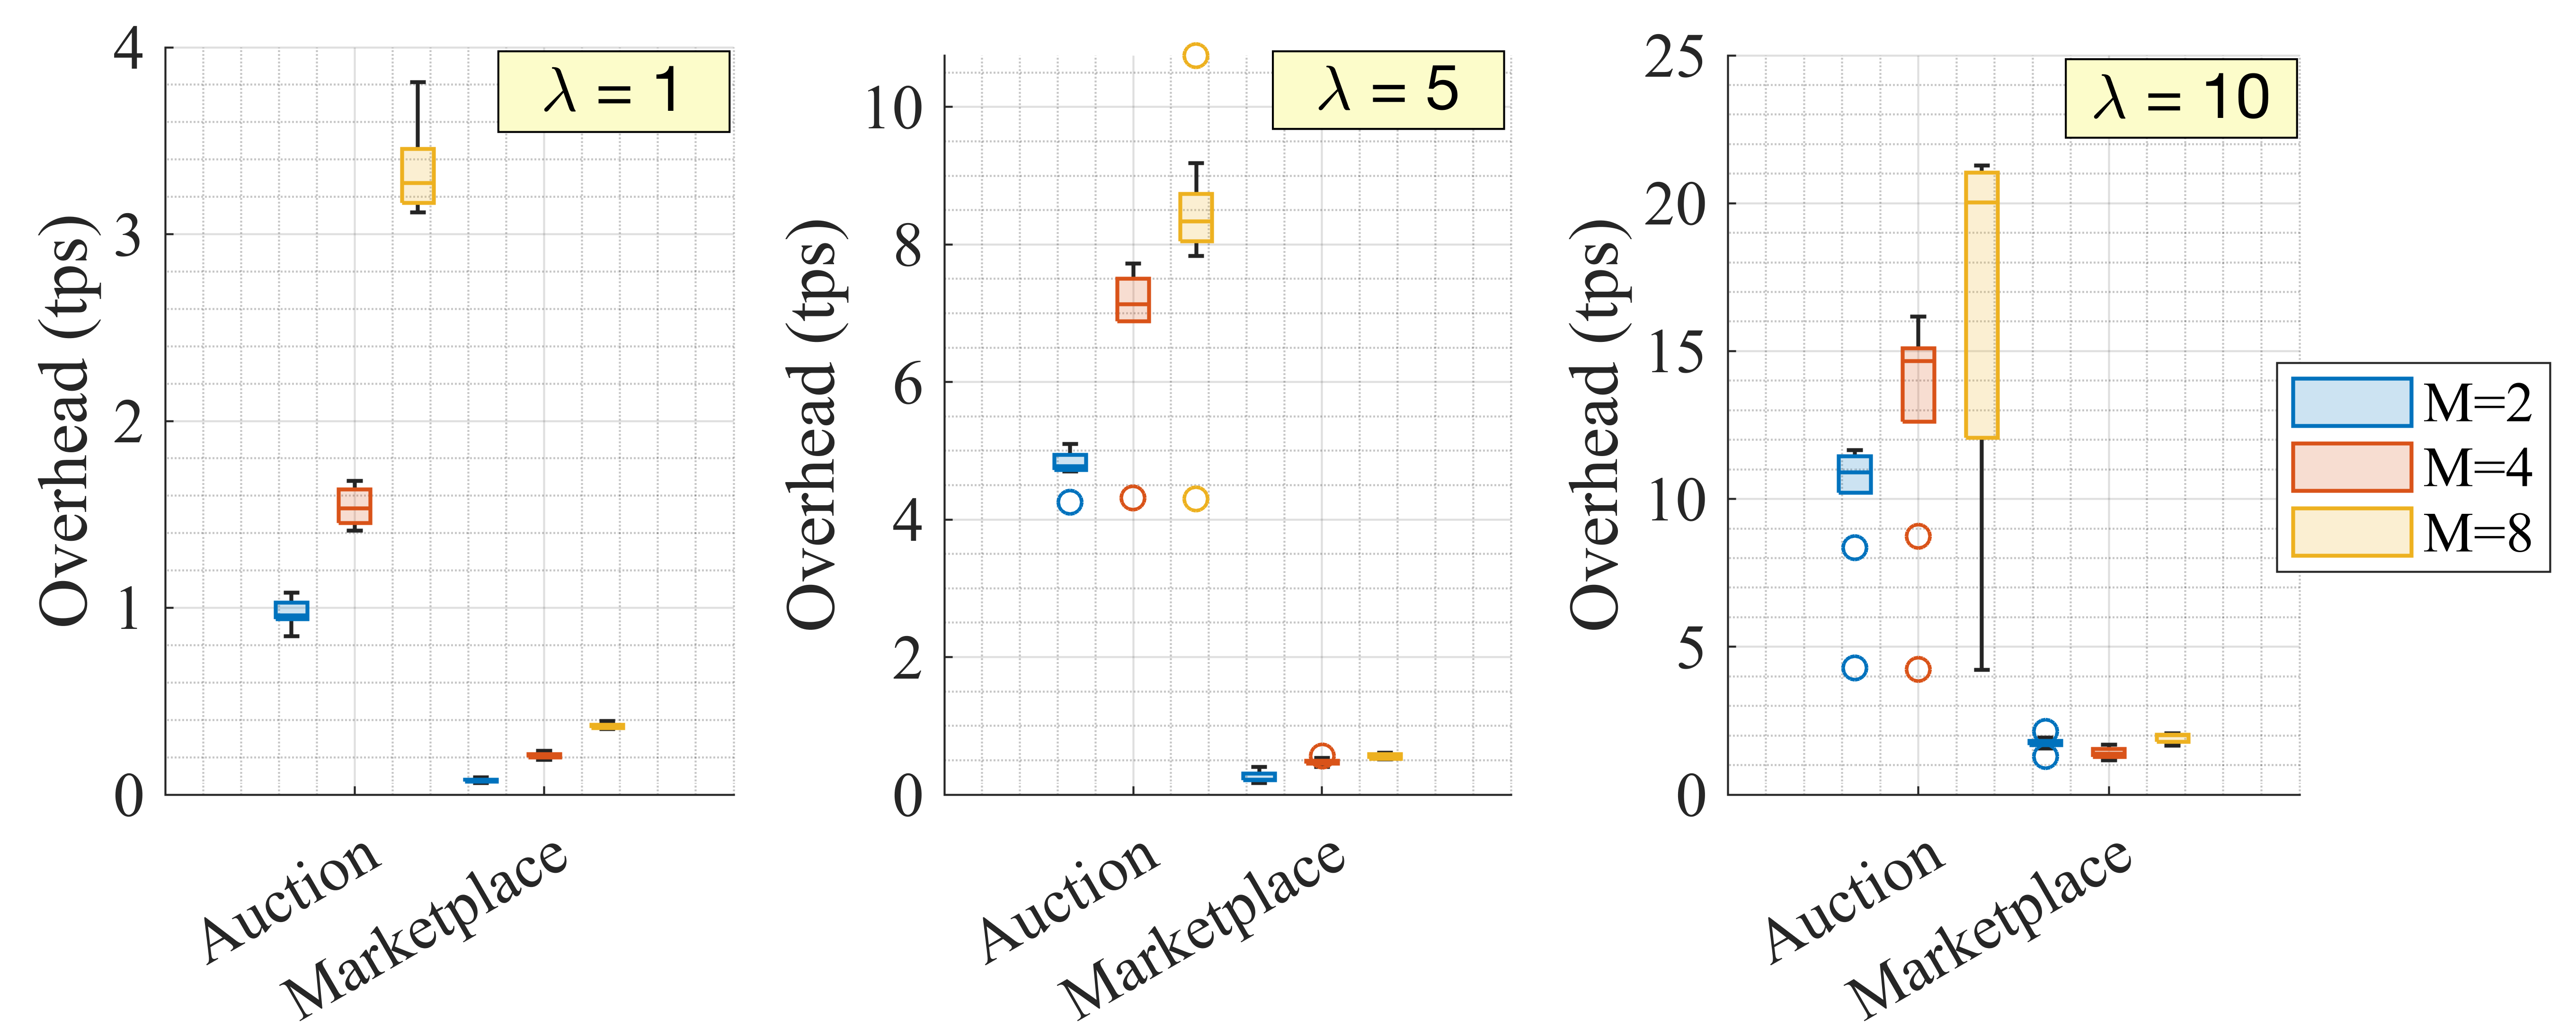
\includegraphics[width=\columnwidth]{boxplot_combined_overhead.png}\label{fig:1}}
%\caption{BC performance for the auction and marketplace-oriented RAN sharing solutions, different block sizes, user arrival rates, and number of operators: a) delay; b) overhead.}
%\label{fig:delay_overhead}
%\end{figure}
We observe that the auction-based mechanism leads to higher delay and overhead than the marketplace approach. The reason is that the auction leads to a higher number of BC transactions, which result from generating tailored service requests and auction bids. This trend is exacerbated as the number of user requests and OPs increases. The marketplace option ensures that the delay and overhead do not increase exponentially with the number of OPs, which makes it a cost-effective solution for automating RAN sharing procedures in future communications systems. Moreover, the marketplace delay decreases with the number of user arrivals, which reduces the waiting time between mined blocks. As for the block size (included in each boxplot), a higher variability is observed in the auction-based approach, which is more susceptible to performance changes for different BC parameters. A more detailed analysis on the impact of BC parameters for communications can be found in~\cite{FWilhelmi_PIMRC}.

%%%%%%%%%%%%%%%%%%%%%%%%%%%%
%% CONCLUSIONS
%%%%%%%%%%%%%%%%%%%%%%%%%%%%
\section{Conclusions}
\label{section:conclusions}

The virtualization of network functions provided by 5G is disrupting the way RAN resources are shared. The O-RAN Alliance is contributing to the development of standards on \textit{intelligent, open, virtualized, and fully interoperable mobile networks}, paving the way to a sharing ecosystem for future RAN with providers operating from the cloud. In such an emerging ecosystem, the advertisement of services and automation of administrative negotiations in the form of an open marketplace may become a fundamental piece to trade resources \textit{as-a-service}. To foster trustworthiness, automation, and an economically driven management of the network, we have proposed to extend the baseline O-RAN architecture with the introduction of a programmable trust concept. To address that, we have envisioned the utilization of BC technology, which is expected to provide trust and traceability to the automation of O-RAN management. The novel O-RAN-based BC-enabled architecture defines new components and procedures to carry out two proposed automated RAN sharing mechanisms, based on auctioning or on an open marketplace. Finally, as a prelude to future research, we have analyzed the main trade-offs offered by the proposed solution through simulation results. We have shown the superiority of the auction and marketplace approaches in terms of capacity, user satisfaction, and efficiency compared to a static solution, at the expense of new overheads and delays introduced by the operation of the BC, which need to be carefully considered in the design of future BC-enabled RAN architectures.

\section*{Acknowledgment}
This work was funded by the IN CERCA grant from the Secretaria d'Universitats i Recerca del departament d'Empresa i Coneixement de la Generalitat de Catalunya, and partially from the Spanish MINECO grant TEC2017-88373-R (5G-REFINE) and Generalitat de Catalunya grant 2017 SGR 1195.
	
\ifCLASSOPTIONcaptionsoff
\newpage
\fi
	
\bibliographystyle{IEEEtran}
\bibliography{bibliography}

% if you will not have a photo at all:
\begin{IEEEbiographynophoto}{Lorenza Giupponi}
(lorenza.giupponi@cttc.es) holds  a  PhD  from  Universitat  Politecnica  de  Catalunya
(2007). She is a Research Director in CTTC, and a member of the CTTC Executive Committee.
\end{IEEEbiographynophoto}
%
\begin{IEEEbiographynophoto}{Francesc Wilhelmi}
(fwilhelmi@cttc.cat) holds a Ph.D. in Information and Communication Technologies (2020), from Universitat Pompeu Fabra (UPF). He is currently a researcher at CTTC. 
\end{IEEEbiographynophoto}

\end{document}